\section{Background: Namecoin}
\label{sec:background}

In this section we cover the background of Namecoin. We begin by looking at the history of the cryptocurrency and then explain why a block chain can be used for our definition of a namespace. We then proceed to discuss the technical design of Namecoin and the mechanisms used in the design. We conclude this section with a discussion about the applications of Namecoin.

{\bf A note about the term `namespace'.} In computer science, a namespace is simply a container for a set of names, so that names in a single namespace must be unique but the same name can exist in different namespaces. We have chosen to use the term in a related but different way: it's a {\em system} that includes client and server software, users, a mechanism, and so on. In fact, Namecoin contains namespaces in the computer science sense, which we term {\em subspaces} in this paper.

\subsection{History}

Namecoin is an alternative cryptocurrency, or altcoin, modeled after Bitcoin \cite{nakamoto2008bitcoin}. Furthermore, it is the first altcoin in the sense that it was the first to create its own block chain, separate from Bitcoin's.  Namecoin shares many similarities with Bitcoin, including the same method for proof-of-work, the same coin cap, the same block creation time, and all of the same transaction operations (with a few additions). Namecoin was inspired after discussions about a BitDNS \cite{bitdns} protocol using a block chain to manage a domain name lookup service. The motivation was that a central authority managing domain names, such as ICANN, requires too much trust in a single entity and represents a single point of failure. The first Namecoin block was mined in April 2011, and as of this writing, over 215,000 total blocks have been mined in the Namecoin system. Because of its similarities with Bitcoin, Namecoin was able to be merge-mined and has been merge-mined with Bitcoin since October 8, 2011 (see the next subsection). 

\subsection{Description of the block chain}
Namecoin is minted and maintained by a decentralized peer-to-peer network.\footnote{This description is adapted from \cite{bonneau2014decentralizing}.}
Namecoin transactions require the digital signature of the account holder to prevent theft, and every transaction is published in an append-only hash chain, called the block chain. The block chain can be extended with new transactions by any participant, and such participants (known as miners) obtain newly minted Namecoin currency (NMC) and transaction fees from the transactions for performing this function. Extensions to the block chain require a proof-of-work that rate-limits the process (to approximately one extension every ten minutes) which enables a steady inflation rate, ample competition among participants to extend the block chain, and adequate time to obtain and verify the history of the block chain for new participants. Informally, the proof-of-work protocol in Namecoin is intended to maintain the following two essential properties about the block chain:

\begin{itemize}

  \item Every party eventually agrees on the order and correctness of transactions in the block chain.
  \item Any party can publish a transaction (for a fee), which will then be verified and, if valid, included in the block chain within a small bounded delay.

\end{itemize}

One use case for a block chain is a tamper-evident log. That is, it can be used as a data structure that stores user-supplied data, and allows users to append data to the end of the log. Each new block has a hash of the previous block, so if data that is earlier in the log is altered, it will be detected. If an adversary wants to tamper with data anywhere in this entire chain, in order to keep the hash pointers consistent, he will have to tamper with the hash pointers all the way up to and including the current block. Thus it emerges that by just remembering the single hash pointer of the head of the chain, users essentially remember a tamper-evident hash of the entire list, all the way back to the genesis block. Namecoin, and all block chain based cryptocurrencies, use this tamper-evident log in order to record all the transactions between users. 


{\bf Block chain security.}
The value and stability of a cryptocurrency are directly related to the amount of proof-of-work involved in the calculations of the blocks because this work is what keeps the data distributed and secure in the tamper-evident block chain. For both Bitcoin and Namecoin, the proof-of-work is shown by calculating the hash of a new block and a random nonce over and over until the calculated hash has a certain number of leading zeros. The number of leading zeros required by the hash is referred to as the difficulty threshold. Namecoin enjoys a very high difficulty threshold for the proof-of-work because it is similar to Bitcoin and supports ``merge mining'' with Bitcoin. This means that miners who are mining Bitcoin can also choose to mine Namecoin at the same time with no extra work. Essentially, this is because the miner is using their computational power to solve a cryptographic puzzle that satisfies the proof-of-work for both block chains at the same time. This is advantageous for the miners because they are rewarded with coins from both systems, and helps Namecoin because it gives the Namecoin network a vastly increased amount of hash power over what it would have if it did not support merged mining.
Including the merge miners, Namecoin has aproximately one third the hash rate of Bitcoin. This provides resilience to a 51\% attack, although a sufficiently large Bitcoin mining pool could still execute this attack.

\subsection{Technical details of names}
\label{subsec:technical_details_of_names}

In this subsection and the next, we present details of Namecoin, separating the technical solution from the mechanism design choices. 

The feature that separates Namecoin from Bitcoin is that Namecoin is a namespace, and can be used to register name/value pairs that can be stored in the block chain and traded amongst individuals. This registration is done using the three script operations exclusive to Namecoin: {\tt NAME\_NEW}, {\tt NAME\_FIRSTUPDATE}, and {\tt NAME\_UPDATE}. In order to understand the registration process, we think it is helpful to walk through the registration process of {\tt name}, roughly following Figure \ref{fig:registration}. 

{\bf NAME\_NEW.}
To start, the user will need to select a coin to be crafted into a token (or special coin) that represents a name and whose value can be changed by whoever possess the token. The next step to register a name is to make a transaction that uses the {\tt NAME\_NEW} script operation in a transaction sending the token from one of their addresses to another. Using {\tt NAME\_NEW}, a user can indicate an interest in {\tt name} for a name/value pair by posting a hash commitment of the desired {\tt name} in the scriptPubKey of the transaction. The reason the user posts the name in hashed form first, rather than in plaintext, is to prevent front-running, which we will explain in Section \ref{sec:design}.
The {\tt NAME\_NEW} operation acts as a signal in the block chain for name parsers to indicate that the next part of the scriptPubKey will be the hash commitment to a name. 
%The protocol then places an {\tt OP\_2DROP} on the stack to remove all of the name information put on the stack with the {\tt NAME\_NEW} operation so that the rest of the locking portion of the scriptPubKey can function just as it does in Bitcoin. 

\begin{figure*}
  \centering
  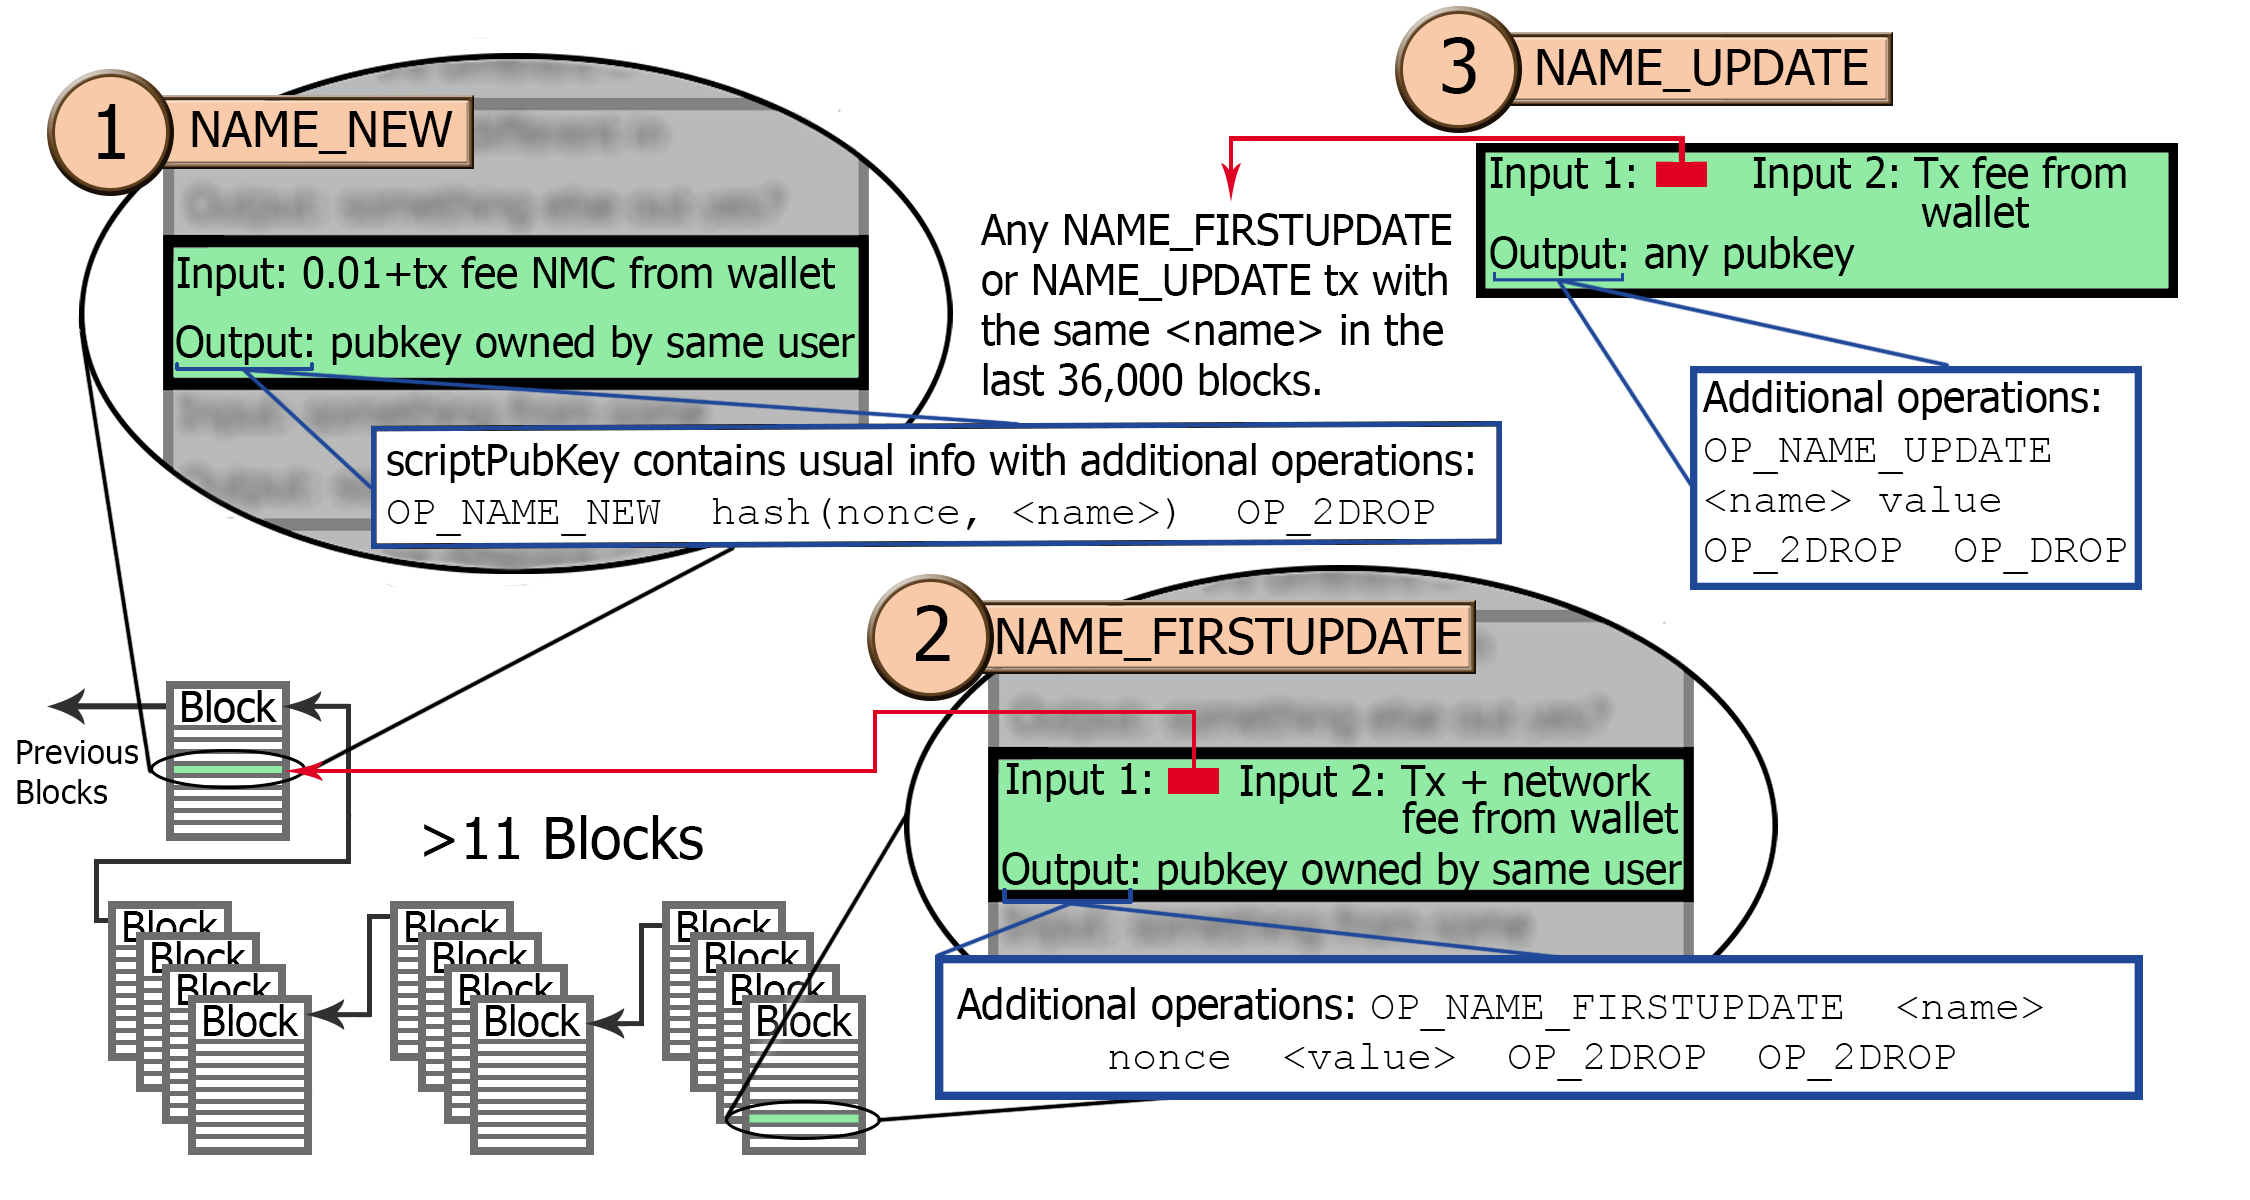
\includegraphics[width=0.95\textwidth]{figures/registration.png}
  \caption{Namecoin name registration protocol described in Section \ref{subsec:technical_details_of_names}}
  \label{fig:registration}
\end{figure*}

{\bf NAME\_FIRSTUPDATE.}
After doing this, and waiting for 12 or more blocks on top of the one containing the {\tt NAME\_NEW} transaction (to ensure that the block chain reaches consensus on the {\tt NAME\_NEW} transaction), the same user can use the output of the {\tt NAME\_NEW} transaction as the input for the {\tt NAME\_FIRSTUPDATE} transaction. Once completed, this will associate the chosen {\tt name} with {\tt value} selected by the user. Similar to {\tt NAME\_NEW}, {\tt NAME\_FIRSTUPDATE} allows data to be posted in the block chain as part of the scriptPubKey of a special transaction. 
To create a {\tt NAME\_NEW} transaction, a user will select, as input, the output of the {\tt NAME\_NEW} transaction. They will then use another address they control as the output for the transaction. The scriptPubKey of this transaction will contain a {\tt NAME\_FIRSTUPDATE}, the {\tt name} desired, the random nonce used in the {\tt NAME\_NEW} hash commitment, and the first {\tt value} for the name to take.\footnote{There are also other operations that exist for reasons of compatibility with Bitcoin; this seems to exist to minimize changes to Bitcoin's script handling code.} 
In order for this transaction to be valid, a miner will verify that the {\tt name} and the provided nonce do, in fact, hash to the commitment in the appropriate {\tt NAME\_NEW} transaction. The output of this transaction now contains the token representing the name/value pair for {\tt name} and {\tt value}, and whoever can unlock and spend the output can utilize the final new operation, {\tt NAME\_UPDATE}.

{\bf NAME\_UPDATE.}
The third and final new operation in Namecoin is the {\tt NAME\_UPDATE} operation. Again, this operation's arguments (the {\tt name} and {\tt newValue}) are stored in the scriptPubKey of a special transaction. This transaction must have as input a {\tt NAME\_FIRSTUPDATE} or {\tt NAME\_UPDATE} output with the same {\tt name}. This operation has three uses: updating, renewing and trading a name. If the user wants to change the {\tt value} associated with a given {\tt name}, they will update {\tt name} with this operation, providing a {\tt newValue}. If names can expire, as they do in Namecoin, then this operation can also be used to renew a name by providing a {\tt newValue} that is the same as the old {\tt value}. In either of these cases, the user will use an address they control as an output of the transaction. The final reason to make a {\tt NAME\_UPDATE} transaction is to trade the special coin to another user. In this case, the user will put, as an output, one of the other user's addresses instead of their own. Once the transaction resolves, the other user will have control over the special coin and can change the value to whatever they deem fit. Because the ownership of {\tt name} is associated with the ownership of the special coin, if the buyer is paying for the name with Namecoins, the exchange between the payment and the name can be atomic (meaning they happen in the same transaction and either are only valid if the other is as well). 

\subsection{Mechanism design}


{\bf Fees.}
Namecoin has been implemented with various fees and protocols to incentivize the behaviors of the users. The special token used in the {\tt NAME\_NEW} transaction has a value of 0.01 NMC. This coin will be not be spendable like other Namecoins while it has a name attached to it. For all of the transactions, {\tt NAME\_NEW}, {\tt NAME\_FIRSTUPDATE}, and {\tt NAME\_UPDATE}, the default behaviour is to have the user pay a transaction fee to the miner. The current expected transaction fee, which is programmed into the Namecoin client, is 0.005 NMC on each transaction. Historically, Namecoin also had a network fee attached to the {\tt NAME\_FIRSTUPDATE} transaction. The network fee is different from the transaction fee; the transaction fee is paid to the miners, whereas the network fee was destroyed (with an {\tt OP\_RETURN}) when a {\tt NAME\_FIRSTUPDATE} transaction was confirmed. The network fee varied over time-- it started at 50 NMC at the genesis block, but decreased by a factor of 2 every 8192 blocks (which is approximately 2 months). The purpose of the network fee was to have a large initial cost to claiming names to deter users from quickly claiming all the desirable names, but then decay off so that eventually the cost of registering a name becomes negligible. As of block 85585, the network fee became small enough that it rounds to 0 and is no longer added onto the transaction. The current implementation of Namecoin has no fees other than the transaction fees and the investment of the token coin.

{\bf Expiration.}
Namecoin has an expiration time for names. Originally, the time period for a name to expire was 12,000 blocks, but by March 2012, the expiration period was increased to 36,000 blocks (which comes out to about 250 days). If a particular {\tt name} hasn't been mentioned in a {\tt NAME\_FIRSTUPDATE} or {\tt NAME\_UPDATE} in 36,000 blocks, the name becomes available again for any user to claim with {\tt NAME\_NEW} and {\tt NAME\_FIRSTUPDATE}. Similarly, a {\tt NAME\_UPDATE} must cite a {\tt NAME\_FIRSTUPDATE} or {\tt NAME\_UPDATE} that is less than 36,000 blocks old as input.

{\bf Changing the protocol.}
Changing the protocol in a cryptocurrency requires a ``hard fork'' or a ``soft fork'' depending on the extent of the change. In a mature system like Bitcoin, this is very difficult. In a fledgling system like Namecoin, however, it is much easier has happened multiple times. Both the addition of merge mining with Bitcoin, and the increase in expiration length were not initially in the design of Namecoin and required hard-forking changes. In order to make these changes, the Namecoin community decided on arbitrary blocks at which point the new protocol would be enforced. Explicitly, up to block 19,199 blocks that were merge mined with Bitcoin were not allowed into the Namceoin block chain, but starting on block 19,200 they were. 
 
\subsection{Applications}

There are many different subspaces in Namecoin, and the different subspaces correspond to applications. When claiming a name, a user prepends the name with a subspace ID and a slash. Namecoin was created to be very general so that it would be useful for any application that would benefit from an online name/value store. While {\tt d/} has the most registered names, there are many used subspaces in Namecoin. The separation of namespaces is not enforced by the protocol in any way, but merely agreed upon by consensus of all users, analogous to open web standards.

{\bf .bit Domains.}
The vision for Namecoin was to use one of these subspaces for DNS lookup in the .bit TLD. Explicitly, Namecoin names associated with .bit domains are prepended with the subspace ID {\tt d/}. If a user wanted the domain example.bit, they would claim the name {\tt d/example}. The owner of example.bit would then set the value to their server address in a way that would be understood by .bit compliant DNS servers as described in the .bit specification \cite{bitdnsspec}.

Most major web servers, such as Apache, ngnix, and lighthttpd will accept connections through .bit domains with minor modifications to their per-site configuration files.

There are a number of ways to resolve .bit domains to IP addresses with varying levels of security. The most secure option is running local DNS resolution software. The three major projects created for this purpose are NMControl \cite{nmcontrol}, a local DNS server, FreeSpeechMe \cite{freespeechme}, a Firefox add-on, and DNSChain \cite{dnschain}, another browser extension. NMControl and FreeSpeechMe both hold a local copy of the block chain and query it for values associated with .bit domains. They parse the value of the name using the specification and seamlessly direct the user to the resolved IP address.

There are a couple less secure options to access .bit domains. Users can connect to specific DNS servers such as OpenNic \cite{opennic} which support resolving .bit domains. However this requires trusting that the DNS server is working properly and accurately reporting results. A final option is using a proxy server hosted in a standard TLD. This requires no local configuration, but users must go to example.bit by visiting example.bitproxy.com.

{\bf OneName.}
The name/value data store in Namecoin has applications beyond DNS. OneName is an online identity service that runs on top of Namecoin, making use of the data store. OneName is a centralized service, but one can use other clients to interact with the block chain in a way that's interoperable with OneName. The idea behind OneName is that a user can have a name/value pair in the block chain that associates said name with different online identities such as an email, GitHub, Twitter, and Bitcoin address. A OneName user can then confirm ownership of accounts on any of these services by referencing their OneName name through some messaging channel in each respective system. For example, if Alice wants to tie her twitter username to her OneName username, she must tweet the message ``Verifying that +Alice is my openname (my Bitcoin username). {\tt https://onename.com/Alice}''. This is similar to the verification scheme Keybase \cite{keybase} uses. A OneName account also has an associated Bitcoin address so users can easily find an address to use to send Bitcoins to a particular individual, if they want.

In order to make a OneName identity, a user can visit OneName's website to create an account. A user makes an account by selecting a username and then optionally entering in their actual name, their account names, a short biography and picture, and a Bitcoin address. OneName takes the information given to it and automatically puts it into a name/value pair, with the name equal to the selected username, and the value containing all the other data. If the username is not already claimed by some user in the Namecoin subspace {\tt u/}, then OneName posts this pair into the block chain. If it is already taken, the website will ask the new user to select a different username. If a user so desires, they can alternatively manually create a name transaction using the Namecoin client to create a name value pair with a name in the {\tt u/} subspace and a value formatted to match the OneName specifications. To incentivize using their website interface, OneName covers the Namecoin fees for their users. 

